\documentclass[16 pt]{amsart}
\usepackage{amscd,amsmath,amsthm,amssymb}
\usepackage{enumerate,varioref}
\usepackage{epsfig}
\usepackage{graphicx}
\usepackage{tikz}
\usetikzlibrary{graphs,arrows,topaths}
\usepackage{mathtools}
\newtheorem{thm}{Theorem}
\newtheorem{cor}[thm]{Corollary}
\newtheorem{lem}[thm]{Lemma}
\newtheorem{prop}[thm]{Proposition}
\theoremstyle{definition}
\newtheorem{defn}[thm]{Definition}
\theoremstyle{remark}
\newtheorem{ex}[thm]{Example}
\newtheorem{rem}[thm]{Remark}
\numberwithin{equation}{subsection}
\newcommand{\R}{\mathbb{R}}
\newcommand{\Z}{\mathbb{Z}}
\newcommand{\C}{\mathbb{C}}
\newcommand{\Q}{\mathbb{Q}}
\newcommand{\lh}{\lim_{h\rightarrow 0}}
\begin{document}

\title{Midterm Maths 140 Winter 2015 \\ DePaul University\\Dr. Alexander}
\maketitle
You have 90 minutes to complete this exam.  Calculators are allowed, but no other electronic devices are permitted.  Please write all your answers in complete, legible sentences, and show all your work to receive full credit.  There are seven (7) problems here.  You may choose to do any 6 of them.  
\vspace{1in}


%table
\begin{center}
  \begin{tabular}{ c | c }
    Problem & Score\\
    \hline
    &\\
    1&\\
    &\\
    2&\\
    &\\
    3&\\
    &\\
    4&\\
    &\\
    5&\\
    &\\
    6&\\
    &\\
    7&\\
    &\\
    Bonus&\\
    &\\
    \hline 
    &\\    
    Total& 
 \end{tabular}
\end{center}

\newpage 
Problem 1. Give the proper negation of the statement:
\[
\text{``If Sue is Bob's sister, then George is his cousin."}
\]

\vspace{1in}


Solution:  This is a conditional, and we know formally that the negation of a conditional becomes an ``and not" statement.

\[
\sim(p\rightarrow q)\equiv p\wedge (\sim q)
\]

So our negation is

\[
\text{``Sue is Bob's sister, but George is not his cousin."}
\]

\newpage
Problem 2. Is the following argument valid?  Justify your answer.\\


\begin{itemize}
\item[] Only God can solve the world's problems.\\
\item[] Technology has solved the world's problems.\\
\item[] $\therefore$ Technology is God.
\end{itemize}


\vspace{1in}

Solution: This argument is, in fact, valid by the transitive property.  Let us not let words get in the way of our logical variables.  This argument may or may not be sound.  Of course, the first two premises are questionable, and to some measure unprovable or possibly even unfalsifiable.

Nonetheless, if we had given a similar argument such as

\begin{itemize}
\item[] Only two can be an even prime number.\\
\item[] $n$ is an even prime number.\\
\item[] $\therefore$ $n$ is 2.
\end{itemize}

Then noone would have thought twice about the validity of the argument form.  In this case, the ``only" acts like ``only if" in terms of statement variables and operations.  Thus the ``arrow" from the first statement is reversed.  Formally we had something like this

\begin{eqnarray*}
p & \leftarrow & q\\
r & \rightarrow & q\\
\therefore r & \rightarrow & p
\end{eqnarray*}

which satisfies transitivity easily.


\newpage

Problem 3. Write the proper negation of the following statement:

\[
\forall a,b,c\in\Z \text{, If } a-b \text{ is even, and } b-c \text{ is even, then } a-c \text{ is even.}
\]

\vspace{1in}

Solution: Here must have another conditional with a universal quantifier.  We know that negation exchanges universality with existence and thus formally we have
\begin{eqnarray*}
\sim (\forall a,b,c\in\Z (P(a,b)\wedge P(b,c)) \rightarrow P(a,c)) \\
\equiv \exists a,b,c\in\Z \text{ s.t. } (P(a,b)\wedge P(b,c))\wedge \sim(P(a,c)) 
\end{eqnarray*}

In English: ``There is a triple of integers $a,b,c$ so that the differences $a-b$ and $b-c$ are even, but the difference $a-c$ is not even.

\newpage

Problem 4. Prove the following statement or give a counterexample:

\[
\forall m\in\Z \text{, If } m \text{ is odd, then } 7m+2 \text{ is odd.}
\]

\vspace{1in}

Solution: Suppose $m$ is odd, then by definition there is some $k\in\Z$ so that $m=2k+1$.
Therefore
\[
7m+2 = 7(2k+1)+2 = 14k+9 = 2(7k+4) + 1
\]
Since integers are closed under addition $7k+4$ is an integer (call it $j$) and thus $7m+2$ can be written $2j+1$ and therefore it is an odd integer.

\newpage

Problem 5. Prove the following or give a counterexample:

\[
\text{Let } r,s\in\Q \text{, then } \frac{r^2+s^2}{3}\in\Q.
\]

\vspace{1in}

Solution: Suppose $r,s\in\Q$ Then there exist $a,b,c,d\in\Z$ with $b\neq 0$ and $d\neq 0$ so that
\[
r = \frac{a}{b}, \text{ and } s=\frac{c}{d}
\]

Then by simple algebra
\[
\frac{r^2+s^2}{3} = \frac{a^2d^2 + b^2c^2}{3b^2d^2}
\]

This is a rational number since the numerator is an integer (integers are closed under addition and multiplication) and the denominator is a nonzero integer (integers are closed under multiplication and none of 3,$b,d$ are zero). Therefore $\frac{r^2+s^2}{3}\in\Q$


\newpage

Problem 6. Prove the following statement by contraposition:

\[
\text{If the product of two positive, real numbers is greater than } n,
\]
\[
\text{then at least one of the numbers is greater than } \sqrt{n}.
\]

\vspace{1in}

Solution: Let's first state the contrapositive: Suppose $x,y$ are two positive, real numbers neither of which is greater than $\sqrt{n}$.  Then their product $xy\le n$.\\

This proof is a one liner:
\[
xy \le \sqrt{n}y \le \sqrt{n}\sqrt{n} =n
\]



\newpage

Problem 7. Draw two graphs.  The first should have both an Euler(ian) circuit and a Hamilton(ian) circuit.  The second should have only a Hamilton(ian) circuit, and not an Euler(ian) circuit.
\vspace{1in}

Solution: The first graph is the simplest possible graph which has both circuits.  Consider the circuit, 1,2,3,1.

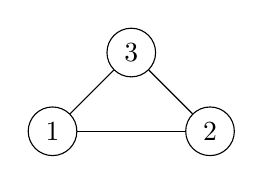
\begin{tikzpicture}
\node[circle, draw] (1) at (0,0){1};
\node[circle, draw] (2) at (2,0){2};
\node[circle, draw] (3) at (1,1){3};
\foreach \from/\to in {1/2,1/3,2/3}
\draw (\from)--(\to);
\end{tikzpicture}

\vspace{.5in}

The second graph has a Hamilton(ian) circuit (1,2,3,4,1) but does not have an Euler(ian) circuit because vertices 1 and 4 have degree 3.

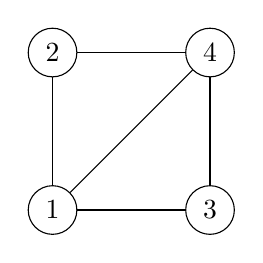
\begin{tikzpicture}
\node[circle,draw] (1) at (0,0){1};
\node[circle,draw] (2) at (0,2){2};
\node[circle,draw] (3) at (2,0){3};
\node[circle,draw] (4) at (2,2){4};
\foreach \from/\to in {1/2,1/3,1/4,2/4,3/4}
	\draw (\from)--(\to);
\end{tikzpicture}

\newpage

Bonus: Is it possible two multiply two large (more than 1,000,000 entries) nonzero matrices together and get a matrix of all zeroes?  For this problem, assume that most of the entries are nonzero.  If not, explain why.  If so, give an example.


\vspace{1in}

Solution: Of course this is possible.  Consider the dot product 
\[
[1,-1,1,-1,\dots] \cdot 
\begin{bmatrix}
1\\1\\1\\ \vdots 
\end{bmatrix} = 0
\]
Now consider two matrices made up of exclusively these vectors to whatever size one desires.

\end{document}